%% LyX 2.0.6 created this file.  For more info, see http://www.lyx.org/.
%% Do not edit unless you really know what you are doing.
\documentclass[english]{report}
\usepackage[T1]{fontenc}
\usepackage[latin9]{inputenc}
\usepackage{geometry}
\geometry{verbose,tmargin=1.5cm,bmargin=1.5cm,lmargin=1.5cm,rmargin=1.5cm}
\setcounter{secnumdepth}{3}
\setcounter{tocdepth}{3}
\setlength{\parindent}{0bp}
\usepackage{float}
\usepackage{graphicx}

\makeatletter

%%%%%%%%%%%%%%%%%%%%%%%%%%%%%% LyX specific LaTeX commands.
%% A simple dot to overcome graphicx limitations
\newcommand{\lyxdot}{.}


\makeatother

\usepackage{babel}
\begin{document}

\title{CRC Tumor Analysis}


\author{Andrew Borgman}

\maketitle

\section*{CRC02}

\begin{center}
% latex table generated in R 3.0.1 by xtable 1.7-1 package
% Tue Aug 27 23:24:15 2013
\begin{table}[ht]
\centering
\begin{tabular}{lll}
  \hline
Model & Comparison & MCMC P-Value \\ 
  \hline
CRC02 & AZD8055 + PD0325901 vs Vechicle & 0.009 \\ 
  CRC02 & AZD8055 alone vs Vechicle & 0.086 \\ 
  CRC02 & BEZ235 + PD0325901 vs Vechicle & 0 \\ 
  CRC02 & BEZ235 alone vs Vechicle & 0.91 \\ 
  CRC02 & PD0325901 alone vs Vechicle & 0.001 \\ 
   \hline
\end{tabular}
\end{table}

\par\end{center}

\begin{center}
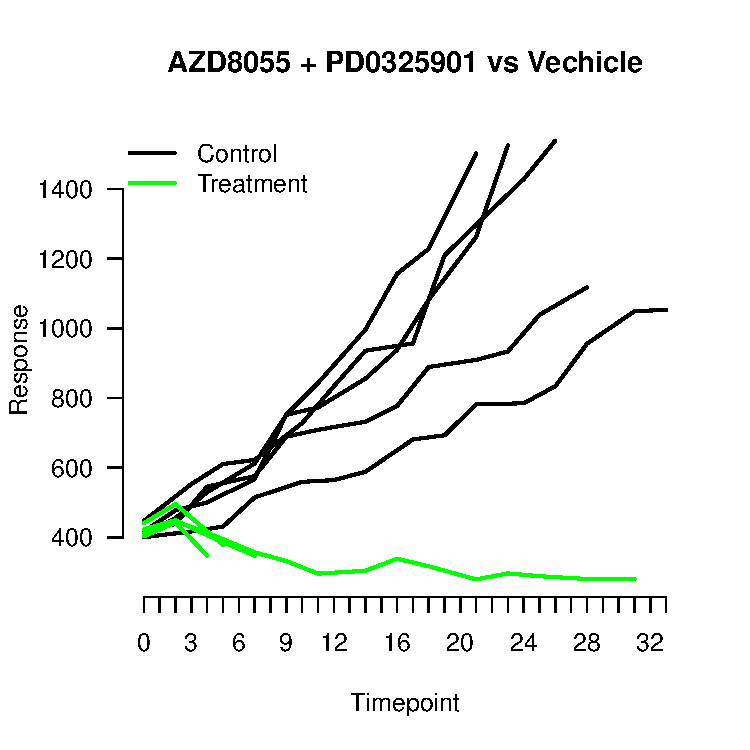
\includegraphics[scale=0.5,bb = 0 0 200 100, draft, type=eps]{/Users/borgmaan/JM_10_CRC/images/treatment_images/CRC02_AZD8055_+_PD0325901_vs_Vechicle.pdf}\hspace{0.5cm}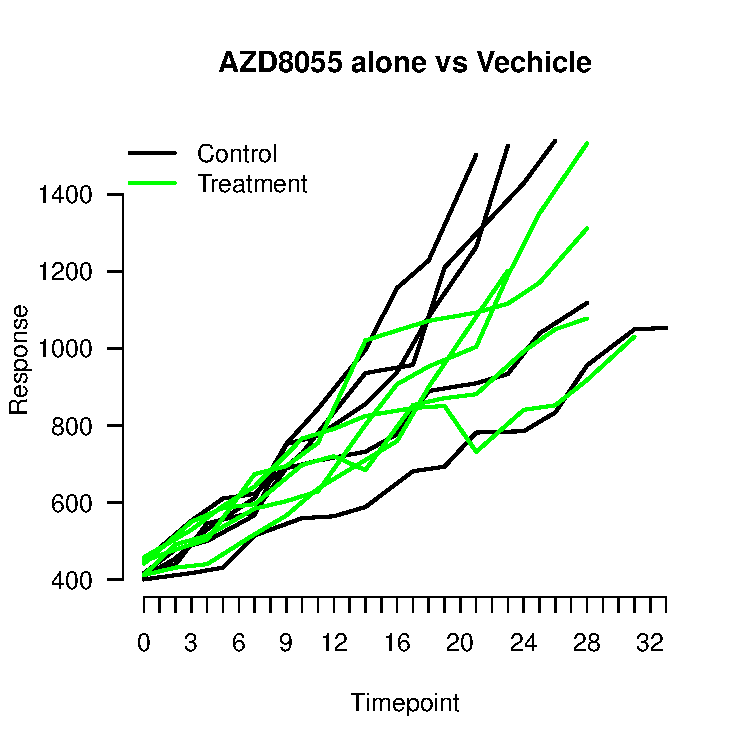
\includegraphics[scale=0.5,bb = 0 0 200 100, draft, type=eps]{/Users/borgmaan/JM_10_CRC/images/treatment_images/CRC02_AZD8055_alone_vs_Vechicle.pdf}
\par\end{center}

\begin{center}
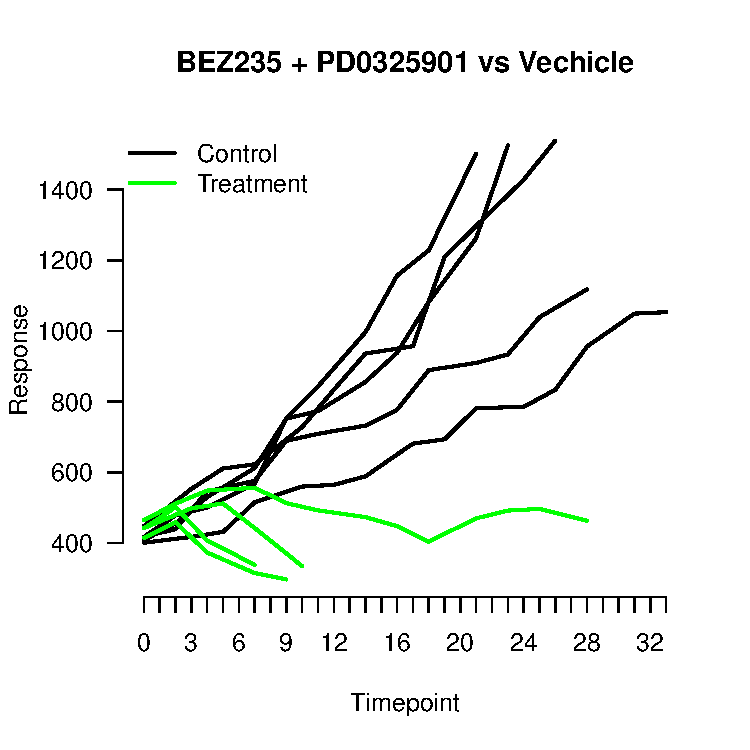
\includegraphics[scale=0.5,bb = 0 0 200 100, draft, type=eps]{/Users/borgmaan/JM_10_CRC/images/treatment_images/CRC02_BEZ235_+_PD0325901_vs_Vechicle.pdf}\hspace{0.5cm}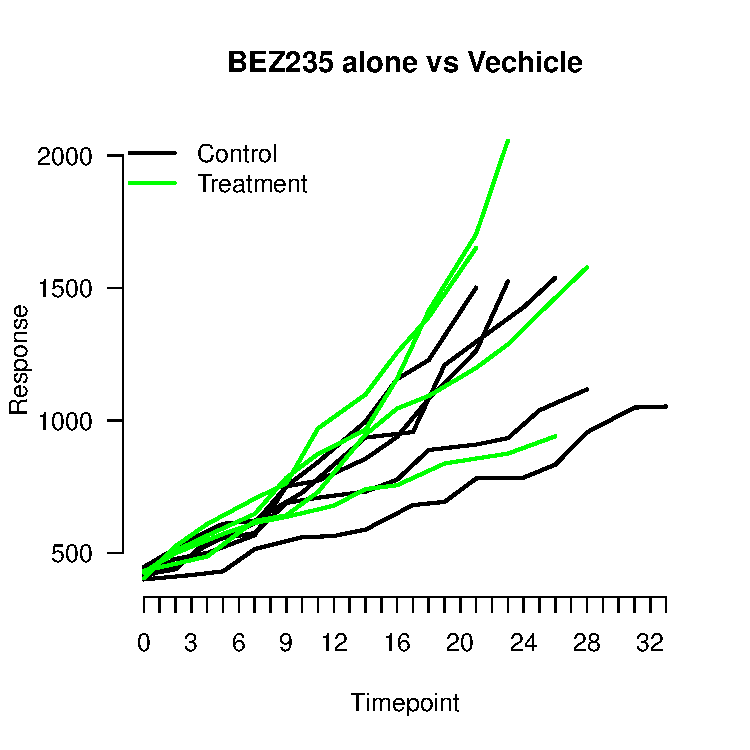
\includegraphics[scale=0.5,bb = 0 0 200 100, draft, type=eps]{/Users/borgmaan/JM_10_CRC/images/treatment_images/CRC02_BEZ235_alone_vs_Vechicle.pdf}
\par\end{center}

\begin{center}
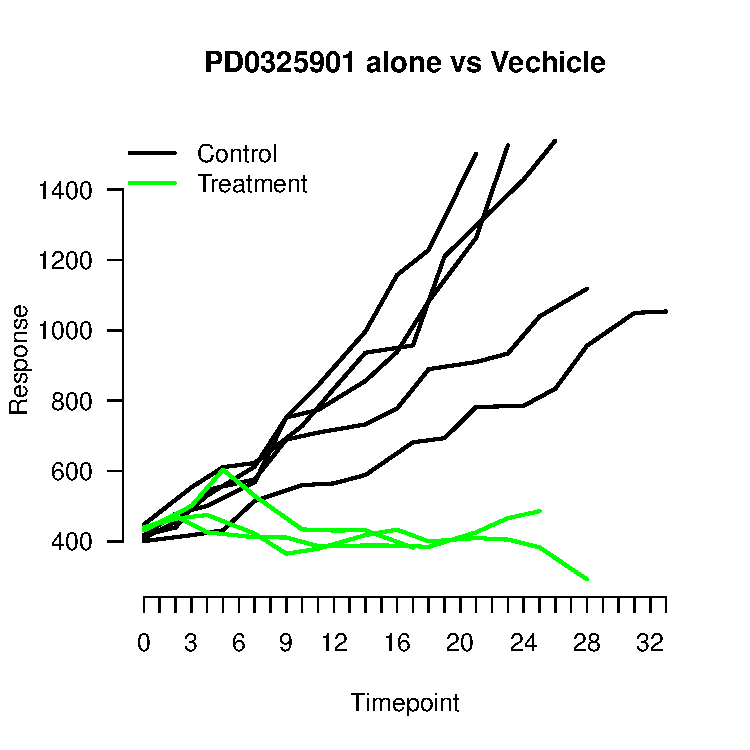
\includegraphics[scale=0.5,bb = 0 0 200 100, draft, type=eps]{/Users/borgmaan/JM_10_CRC/images/treatment_images/CRC02_PD0325901_alone_vs_Vechicle.pdf}
\par\end{center}


\section*{CRC18}

\begin{center}
% latex table generated in R 3.0.1 by xtable 1.7-1 package
% Tue Aug 27 23:24:15 2013
\begin{table}[ht]
\centering
\begin{tabular}{lll}
  \hline
Model & Comparison & MCMC P-Value \\ 
  \hline
CRC18 & AZD8055 + PD0325901 vs Vechicle & 0.021 \\ 
  CRC18 & AZD8055 alone vs Vechicle & 0.228 \\ 
  CRC18 & BEZ235 + PD0325901 vs Vechicle & 0.05 \\ 
  CRC18 & BEZ235 alone vs Vechicle & 0.201 \\ 
  CRC18 & PD0325901 alone vs Vechicle & 0.013 \\ 
   \hline
\end{tabular}
\end{table}

\par\end{center}

\begin{center}
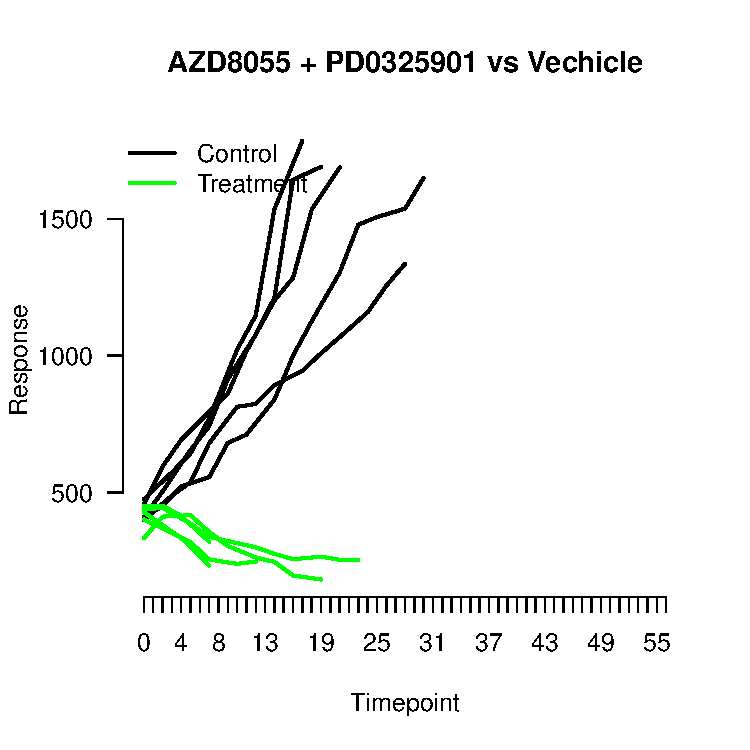
\includegraphics[scale=0.5,bb = 0 0 200 100, draft, type=eps]{/Users/borgmaan/JM_10_CRC/images/treatment_images/CRC18_AZD8055_+_PD0325901_vs_Vechicle.pdf}\hspace{0.5cm}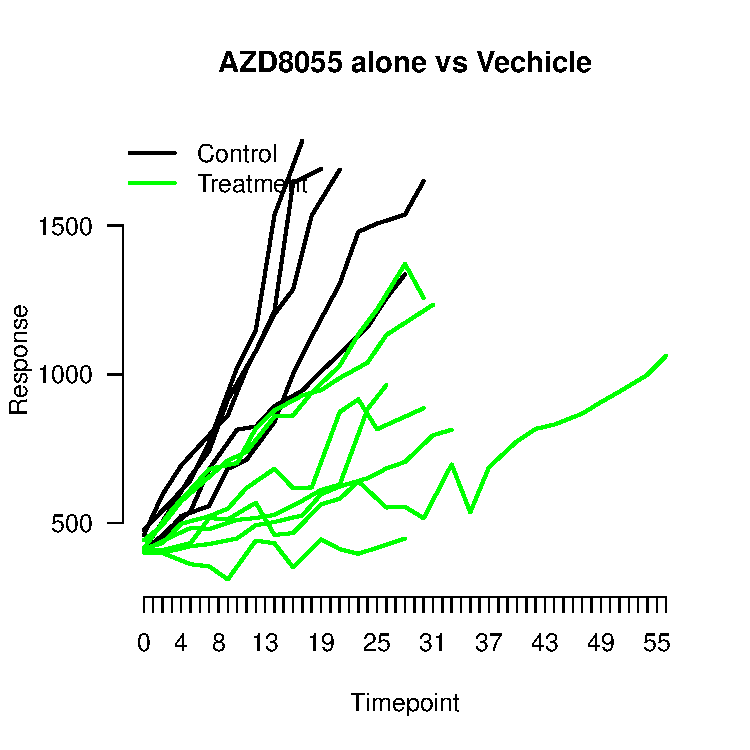
\includegraphics[scale=0.5,bb = 0 0 200 100, draft, type=eps]{/Users/borgmaan/JM_10_CRC/images/treatment_images/CRC18_AZD8055_alone_vs_Vechicle.pdf}
\par\end{center}

\begin{center}
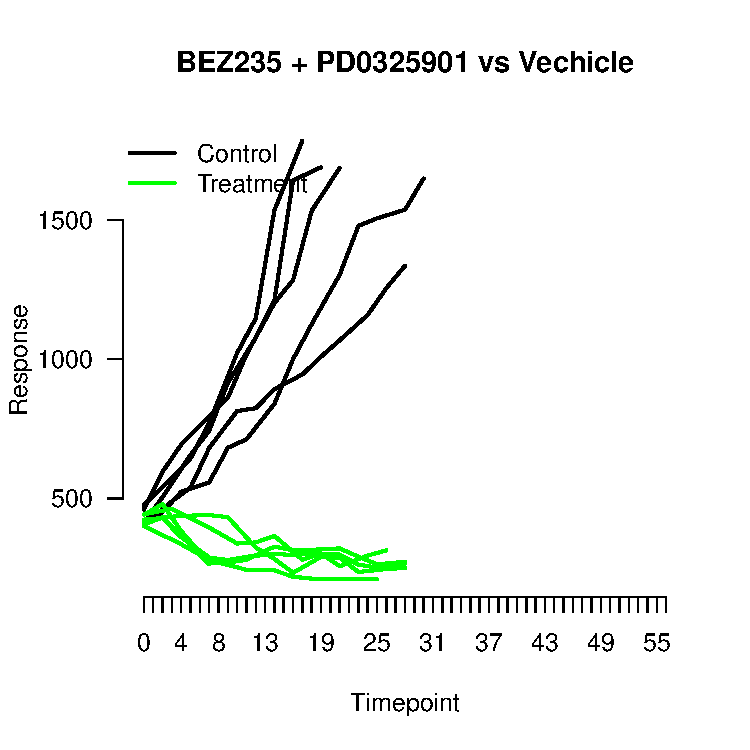
\includegraphics[scale=0.5,bb = 0 0 200 100, draft, type=eps]{/Users/borgmaan/JM_10_CRC/images/treatment_images/CRC18_BEZ235_+_PD0325901_vs_Vechicle.pdf}\hspace{0.5cm}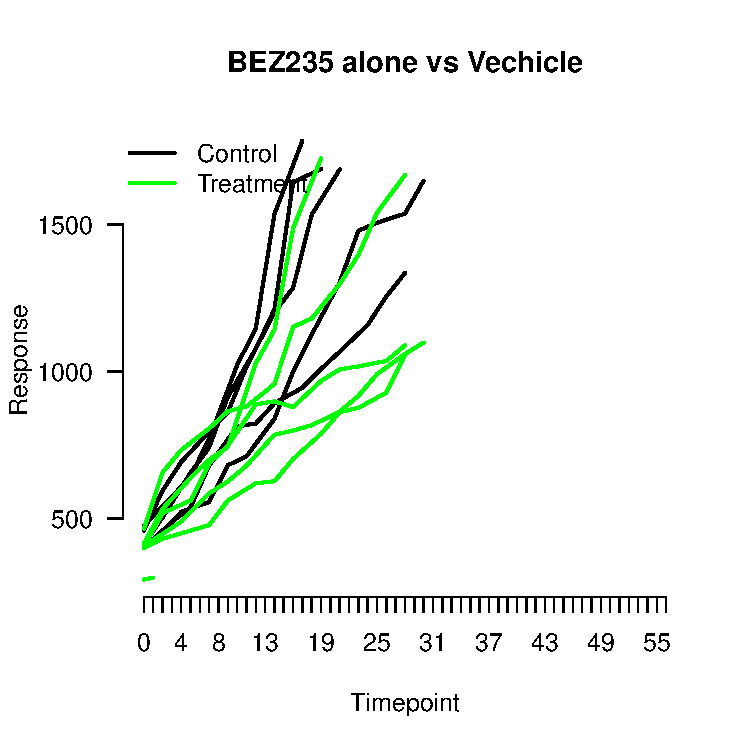
\includegraphics[scale=0.5,bb = 0 0 200 100, draft, type=eps]{/Users/borgmaan/JM_10_CRC/images/treatment_images/CRC18_BEZ235_alone_vs_Vechicle.pdf}
\par\end{center}

\begin{center}
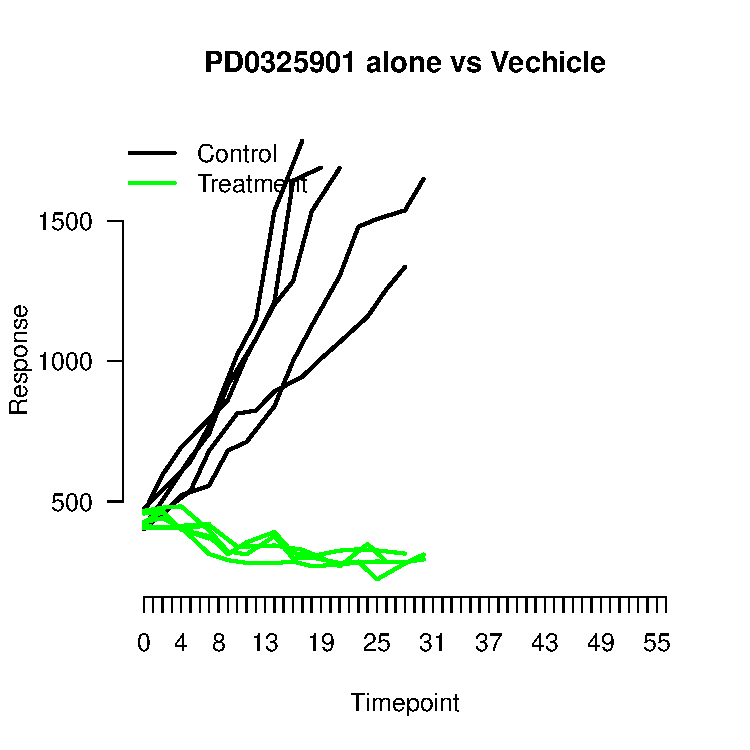
\includegraphics[scale=0.5,bb = 0 0 200 100, draft, type=eps]{/Users/borgmaan/JM_10_CRC/images/treatment_images/CRC18_PD0325901_alone_vs_Vechicle.pdf}
\par\end{center}


\section*{JPM09}

\begin{center}
% latex table generated in R 3.0.1 by xtable 1.7-1 package
% Tue Aug 27 23:24:15 2013
\begin{table}[ht]
\centering
\begin{tabular}{lll}
  \hline
Model & Comparison & MCMC P-Value \\ 
  \hline
JPM09 & AZD8055 + PD0325901 vs Vechicle & 0.263 \\ 
  JPM09 & AZD8055 alone vs Vechicle & 0.293 \\ 
  JPM09 & BEZ235 + PD0325901 vs Vechicle & 0.314 \\ 
  JPM09 & BEZ235 alone vs Vechicle & 0.526 \\ 
  JPM09 & PD0325901 alone vs Vechicle & 0.024 \\ 
   \hline
\end{tabular}
\end{table}

\par\end{center}

\begin{center}
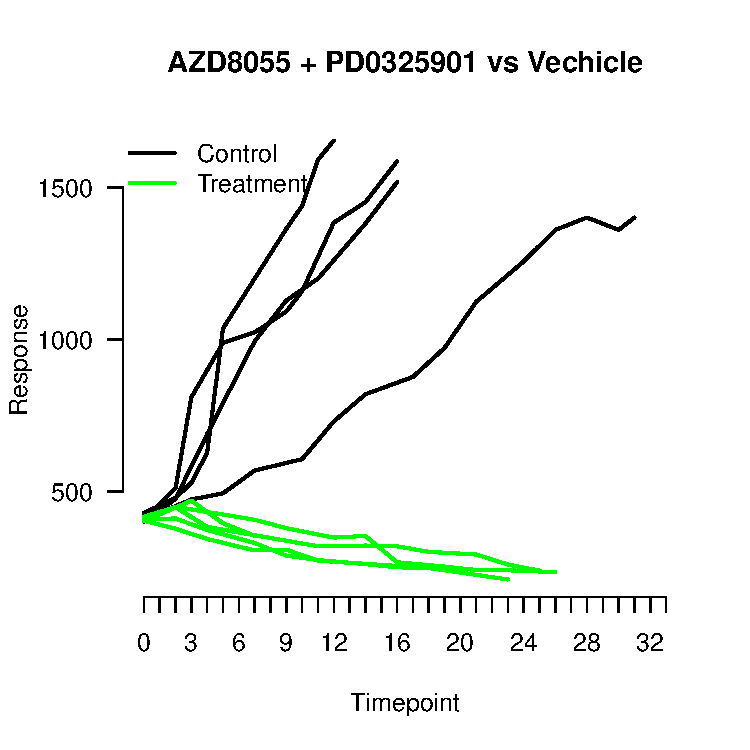
\includegraphics[scale=0.5,bb = 0 0 200 100, draft, type=eps]{/Users/borgmaan/JM_10_CRC/images/treatment_images/JPM09_AZD8055_+_PD0325901_vs_Vechicle.pdf}\hspace{0.5cm}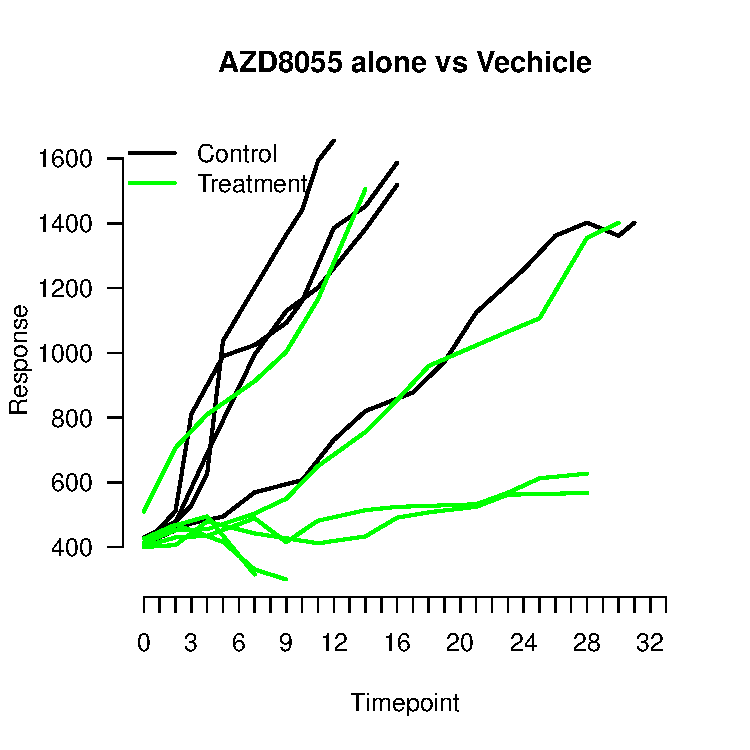
\includegraphics[scale=0.5,bb = 0 0 200 100, draft, type=eps]{/Users/borgmaan/JM_10_CRC/images/treatment_images/JPM09_AZD8055_alone_vs_Vechicle.pdf}
\par\end{center}

\begin{center}
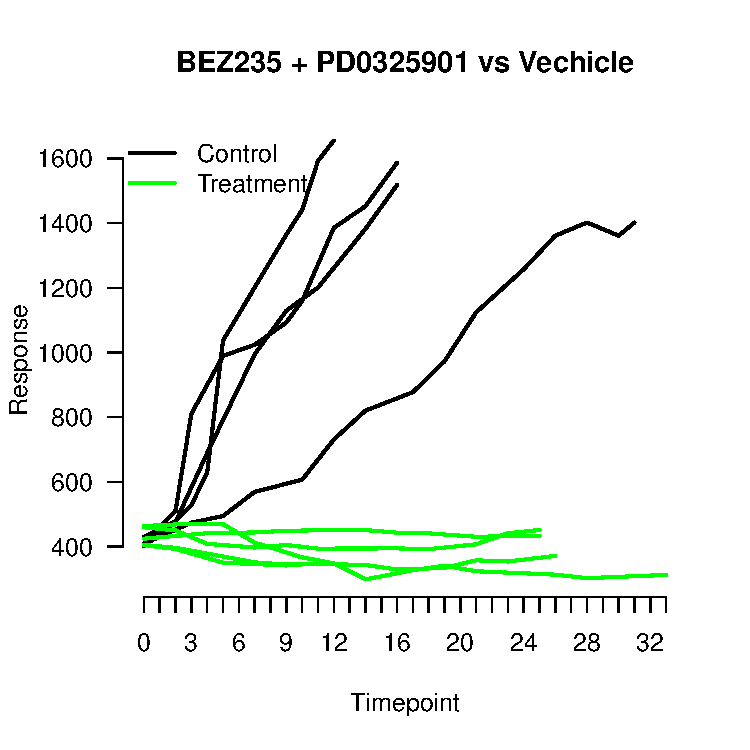
\includegraphics[scale=0.5,bb = 0 0 200 100, draft, type=eps]{/Users/borgmaan/JM_10_CRC/images/treatment_images/JPM09_BEZ235_+_PD0325901_vs_Vechicle.pdf}\hspace{0.5cm}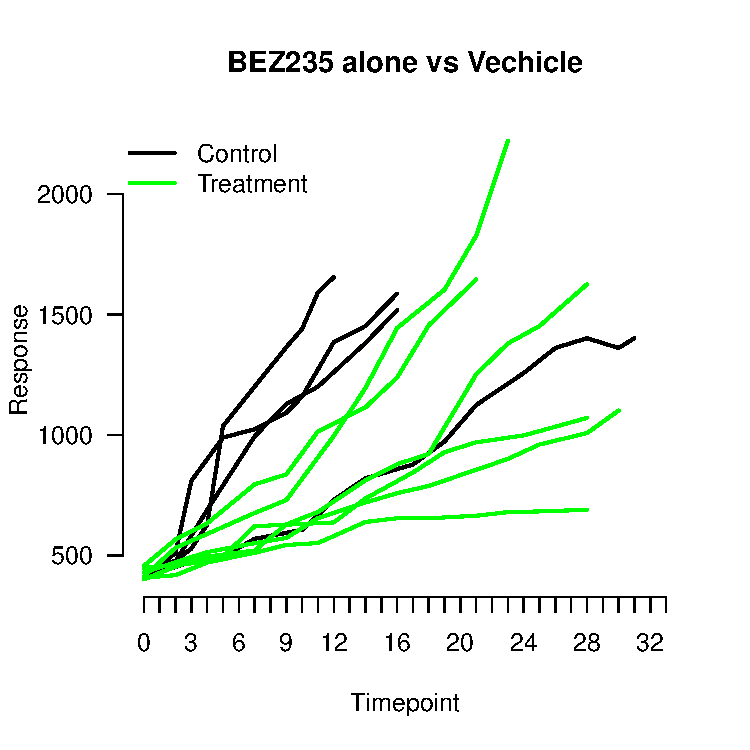
\includegraphics[scale=0.5,bb = 0 0 200 100, draft, type=eps]{/Users/borgmaan/JM_10_CRC/images/treatment_images/JPM09_BEZ235_alone_vs_Vechicle.pdf}
\par\end{center}

\begin{center}
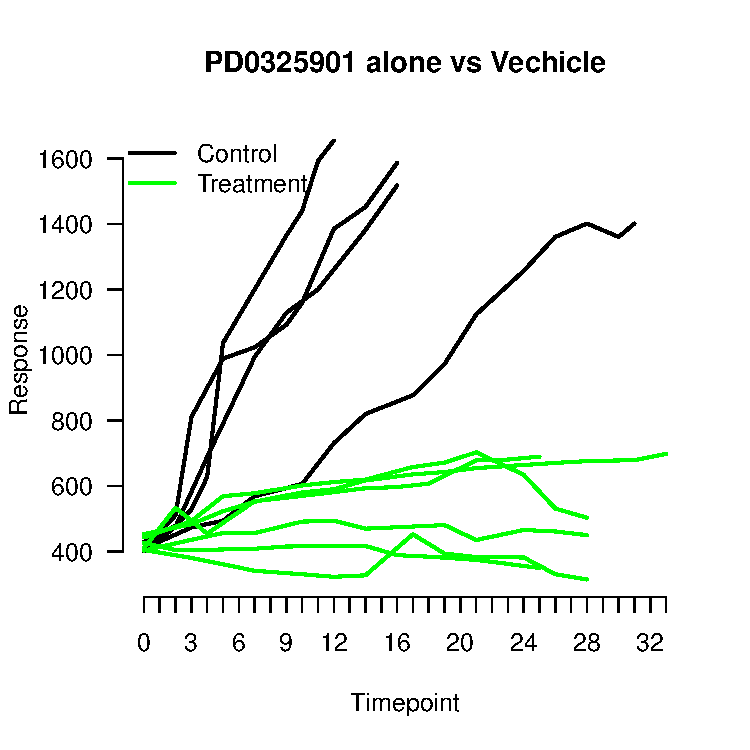
\includegraphics[scale=0.5,bb = 0 0 200 100, draft, type=eps]{/Users/borgmaan/JM_10_CRC/images/treatment_images/JPM09_PD0325901_alone_vs_Vechicle.pdf}
\par\end{center}


\section*{JPM12}

\begin{center}
% latex table generated in R 3.0.1 by xtable 1.7-1 package
% Tue Aug 27 23:24:15 2013
\begin{table}[ht]
\centering
\begin{tabular}{lll}
  \hline
Model & Comparison & MCMC P-Value \\ 
  \hline
JPM12 & AZD8055 + PD0325901 vs Vechicle & 0.25 \\ 
  JPM12 & AZD8055 alone vs Vechicle & 0.436 \\ 
  JPM12 & BEZ235 + PD0325901 vs Vechicle & 0.047 \\ 
  JPM12 & BEZ235 alone vs Vechicle & 0 \\ 
  JPM12 & PD0325901 alone vs Vechicle & 0.387 \\ 
   \hline
\end{tabular}
\end{table}

\par\end{center}

\begin{center}
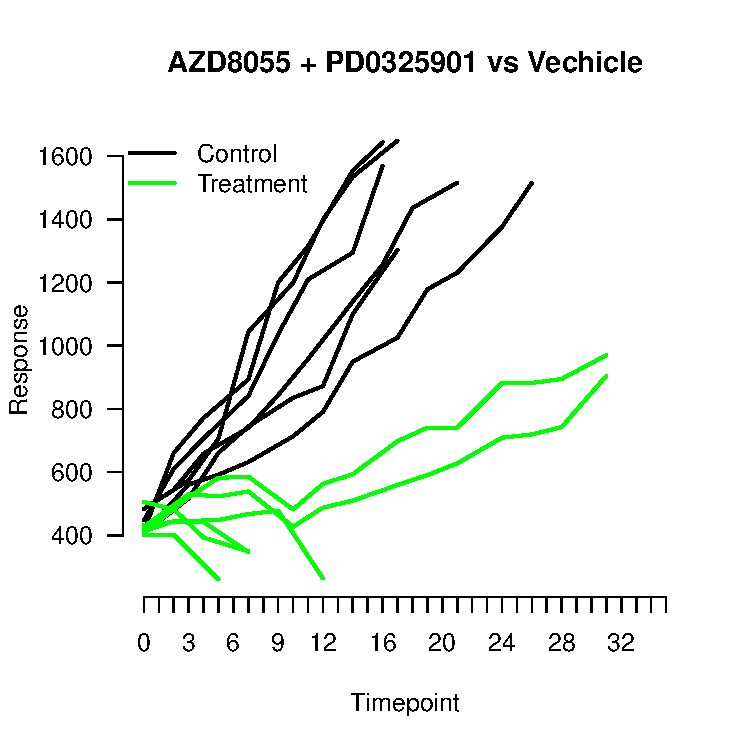
\includegraphics[scale=0.5,bb = 0 0 200 100, draft, type=eps]{/Users/borgmaan/JM_10_CRC/images/treatment_images/JPM12_AZD8055_+_PD0325901_vs_Vechicle.pdf}\hspace{0.5cm}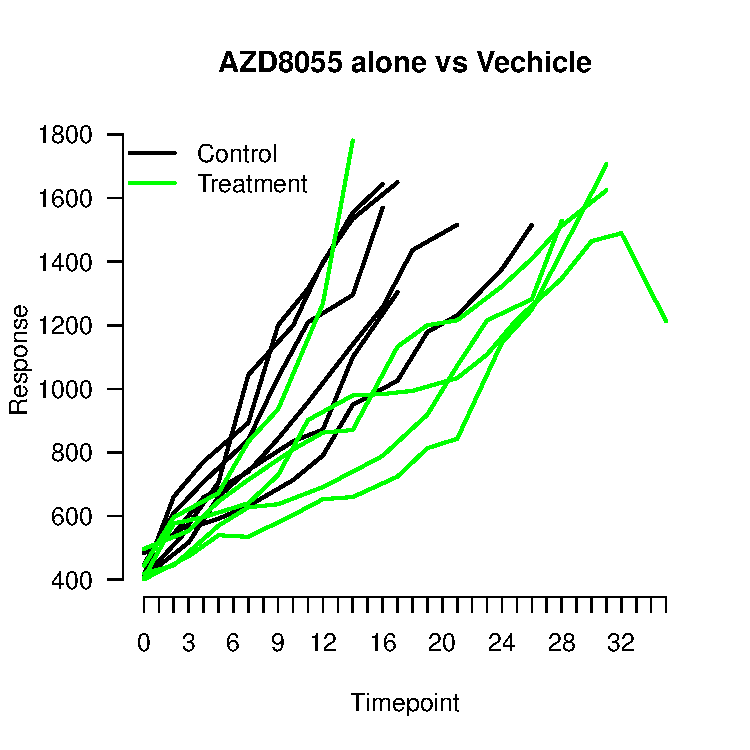
\includegraphics[scale=0.5,bb = 0 0 200 100, draft, type=eps]{/Users/borgmaan/JM_10_CRC/images/treatment_images/JPM12_AZD8055_alone_vs_Vechicle.pdf}
\par\end{center}

\begin{center}
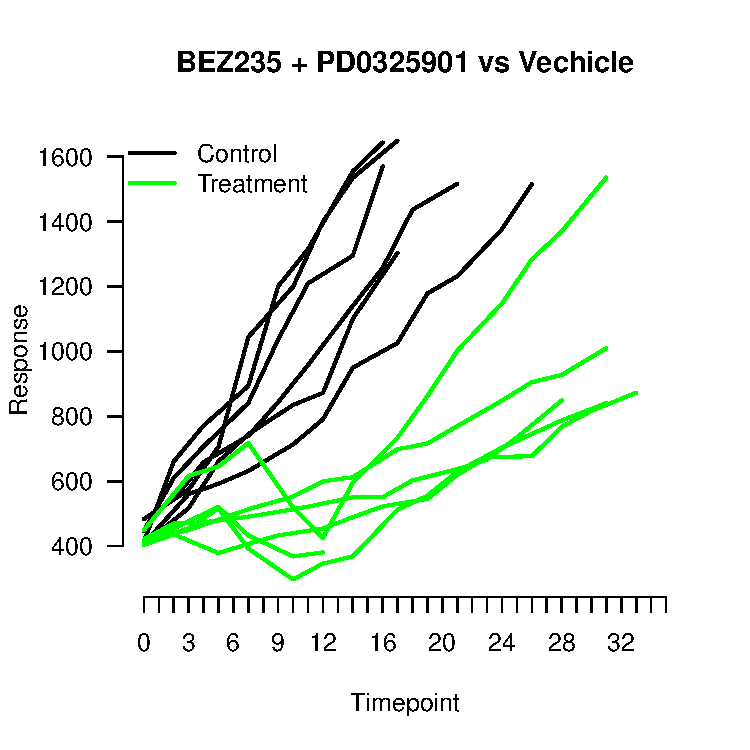
\includegraphics[scale=0.5,bb = 0 0 200 100, draft, type=eps]{/Users/borgmaan/JM_10_CRC/images/treatment_images/JPM12_BEZ235_+_PD0325901_vs_Vechicle.pdf}\hspace{0.5cm}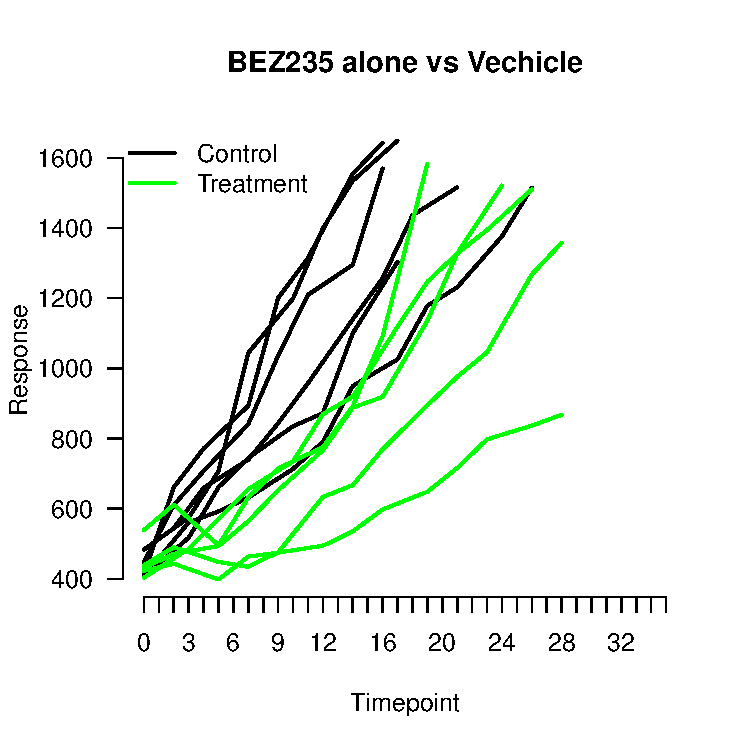
\includegraphics[scale=0.5,bb = 0 0 200 100, draft, type=eps]{/Users/borgmaan/JM_10_CRC/images/treatment_images/JPM12_BEZ235_alone_vs_Vechicle.pdf}
\par\end{center}

\begin{center}
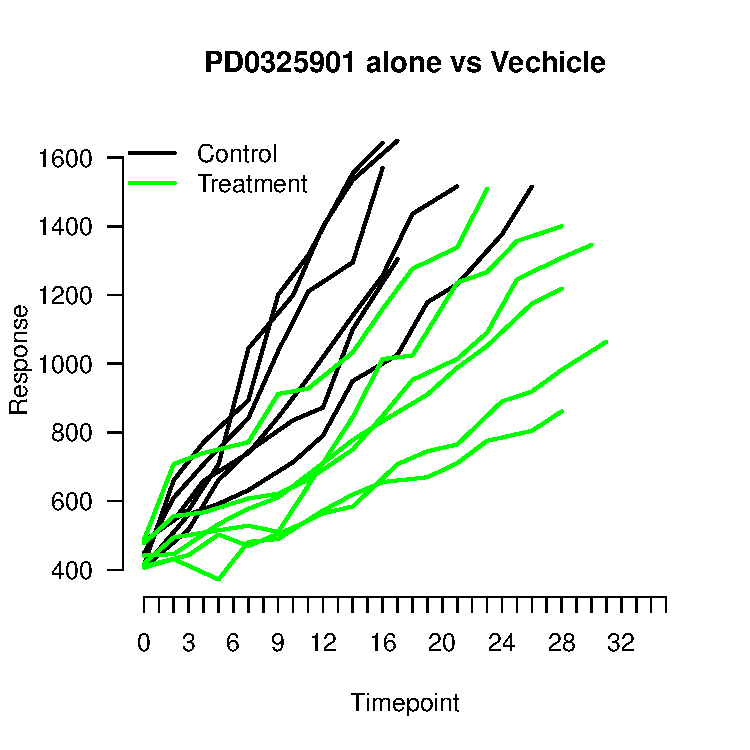
\includegraphics[scale=0.5,bb = 0 0 200 100, draft, type=eps]{/Users/borgmaan/JM_10_CRC/images/treatment_images/JPM12_PD0325901_alone_vs_Vechicle.pdf}
\par\end{center}


\section*{JPM16}

\begin{center}
% latex table generated in R 3.0.1 by xtable 1.7-1 package
% Tue Aug 27 23:24:15 2013
\begin{table}[ht]
\centering
\begin{tabular}{lll}
  \hline
Model & Comparison & MCMC P-Value \\ 
  \hline
JPM16 & AZD8055 + PD0325901 vs Vechicle & 0.141 \\ 
  JPM16 & AZD8055 alone vs Vechicle & 0.713 \\ 
  JPM16 & BEZ235 + PD0325901 vs Vechicle & 0.958 \\ 
  JPM16 & BEZ235 alone vs Vechicle & 0.051 \\ 
  JPM16 & PD0325901 alone vs Vechicle & 0.146 \\ 
   \hline
\end{tabular}
\end{table}

\par\end{center}

\begin{center}
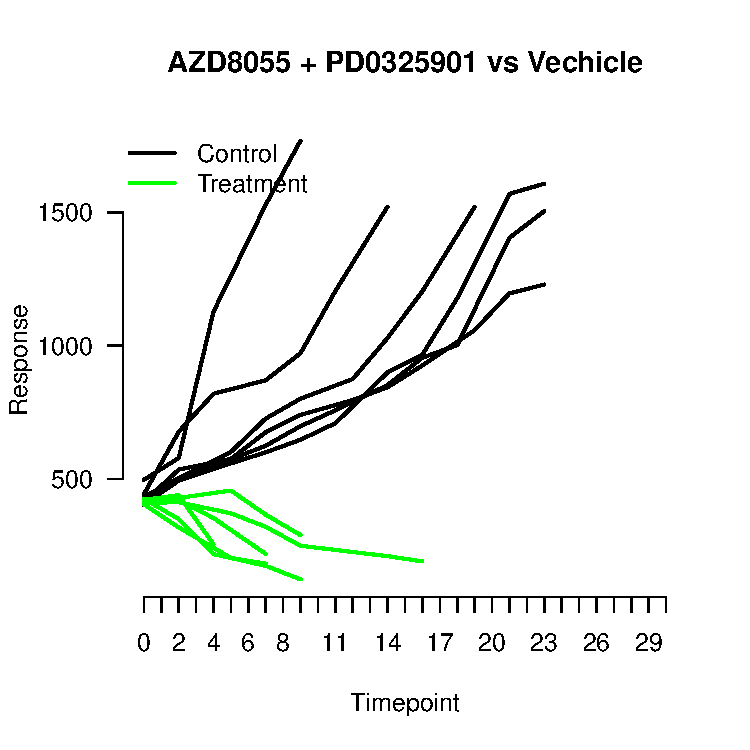
\includegraphics[scale=0.5,bb = 0 0 200 100, draft, type=eps]{/Users/borgmaan/JM_10_CRC/images/treatment_images/JPM16_AZD8055_+_PD0325901_vs_Vechicle.pdf}\hspace{0.5cm}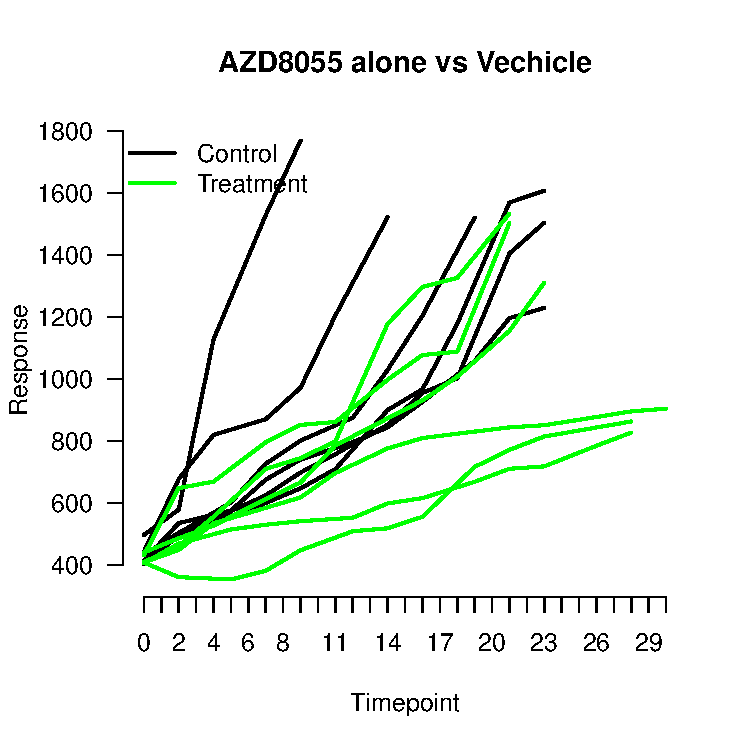
\includegraphics[scale=0.5,bb = 0 0 200 100, draft, type=eps]{/Users/borgmaan/JM_10_CRC/images/treatment_images/JPM16_AZD8055_alone_vs_Vechicle.pdf}
\par\end{center}

\begin{center}
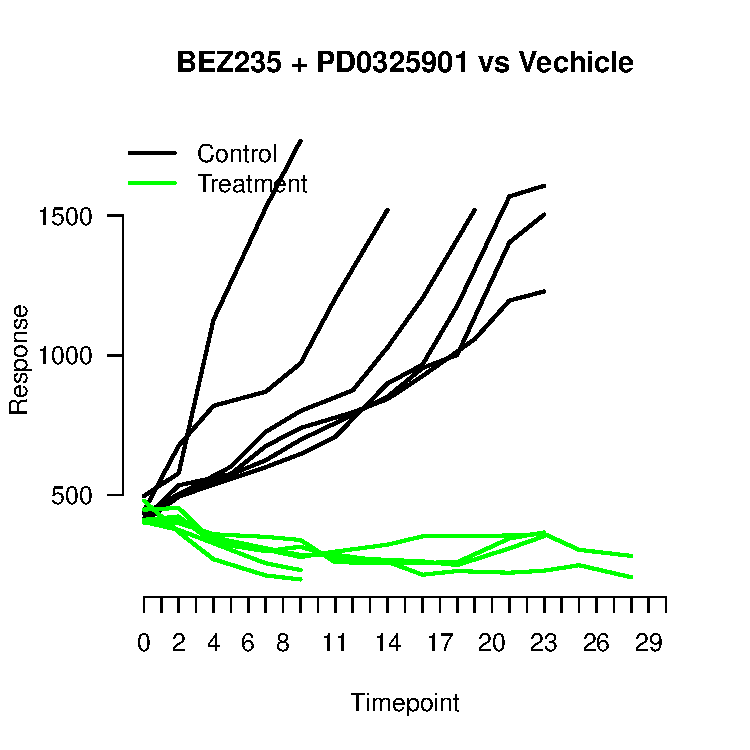
\includegraphics[scale=0.5,bb = 0 0 200 100, draft, type=eps]{/Users/borgmaan/JM_10_CRC/images/treatment_images/JPM16_BEZ235_+_PD0325901_vs_Vechicle.pdf}\hspace{0.5cm}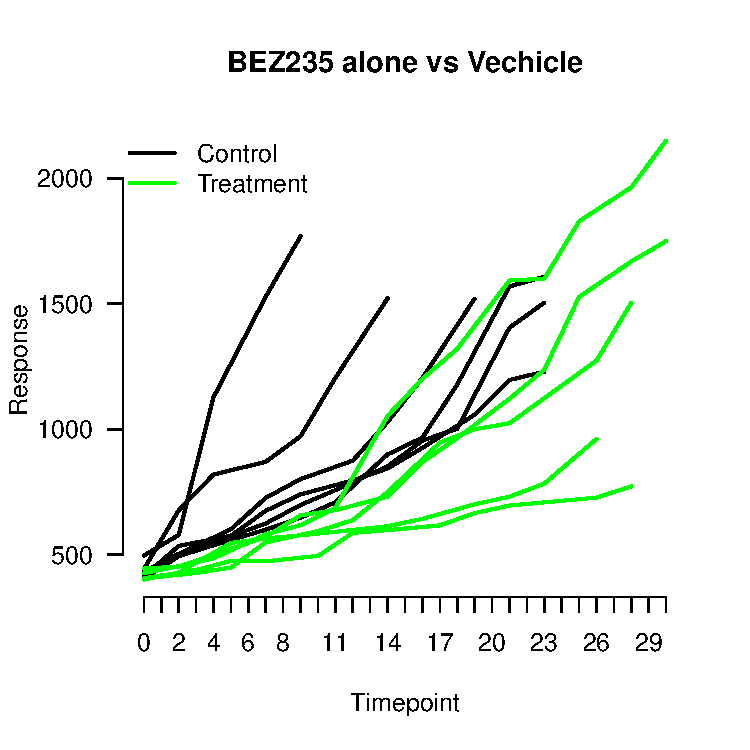
\includegraphics[scale=0.5,bb = 0 0 200 100, draft, type=eps]{/Users/borgmaan/JM_10_CRC/images/treatment_images/JPM16_BEZ235_alone_vs_Vechicle.pdf}
\par\end{center}

\begin{center}
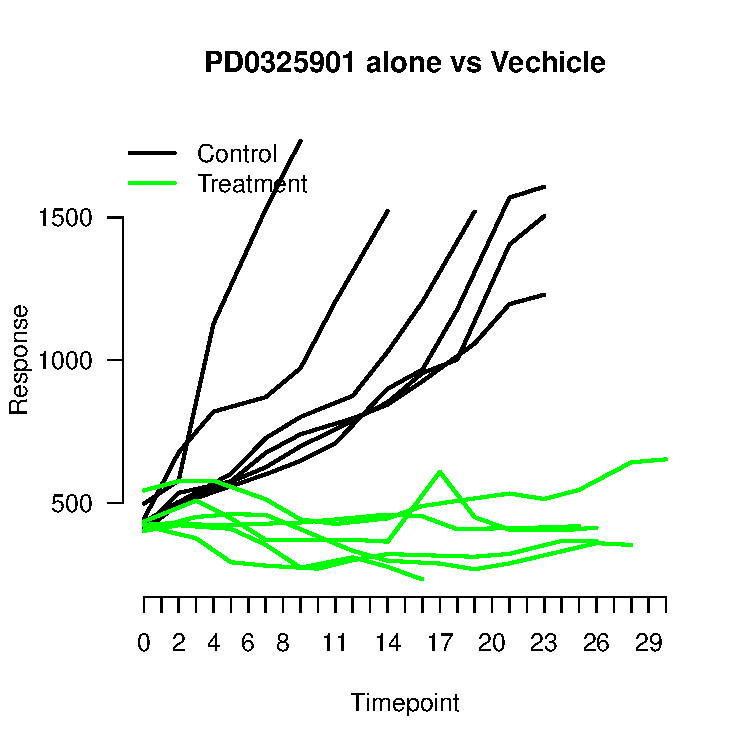
\includegraphics[scale=0.5,bb = 0 0 200 100, draft, type=eps]{/Users/borgmaan/JM_10_CRC/images/treatment_images/JPM16_PD0325901_alone_vs_Vechicle.pdf}
\par\end{center}
\end{document}
